\documentclass[a4paper, 11pt, titlepage]{article}
\usepackage{graphicx}
\usepackage{pdfpages}
\usepackage{fancybox}
\usepackage[francais]{babel}
\usepackage[utf8]{inputenc}
% \usepackage[T1]{fontenc}
\usepackage{amsmath,amsfonts,amssymb}
\usepackage{fancyhdr}
\usepackage{stackrel}
\usepackage{babel,indentfirst}
\usepackage{xspace}
\usepackage{url}
\usepackage{titling}
\usepackage{listings}
\usepackage{color}
\usepackage{array}
\usepackage{hyperref}
\usepackage{makecell}
\usepackage{tikz}
\usepackage{float}
\usepackage{wrapfig}

%\setlength{\parindent}{0pt}
\setlength{\parskip}{1ex}
\setlength{\textwidth}{17cm}
\setlength{\textheight}{24cm}
\setlength{\oddsidemargin}{-.7cm}
\setlength{\evensidemargin}{-.7cm}
\setlength{\topmargin}{-.5in}


\lstset{
  sensitive=f,
  morestring=[d]",
  showstringspaces=false,
  basicstyle=\small\ttfamily,
  keywordstyle=\bf\small,
  commentstyle=\itshape,
  stringstyle=\sf,
  extendedchars=true,
  columns=[c]fixed
}



\predate{
\begin{center}
}
\postdate{
\\
\vspace{1.5cm}

\includegraphics[scale=0.7]{imag.png}
\end{center}}


\title {{ {\huge Compte rendu du projet make }} }

\author{\Large Equipe 10 \\
\\
    {\sc Boudouin}~Philippe\\
    {\sc Danet}~Nicolas\\
    {\sc Ferrand}~Pierre\\
    {\sc Gouttefarde}~Léo
}

\date{Vendredi 25 Novembre 2016}

\lhead{Projet Make}
\rhead{Compte rendu}

\begin{document}
\pagestyle{fancy}
\maketitle

\setcounter{tocdepth}{2}

\tableofcontents
\newpage

\section {Présentation}




\newpage

\section {Tests de performance}

Les tests ci-dessous on été effectués sur les machines du cluster Edel de Grenoble, avec un maximum de 42 machines.

Les caractéristiques de ces machines sont les suivantes :

\begin{itemize}

\item
2 CPUs Intel Xeon E5520

\item
4 coeurs par CPU

\item
24 GB de RAM

\item
119 GB d'espace disque SSD

\end{itemize}



Les tests ont été réalisés en exploitant chacun des 8 coeurs (2 x 4 coeurs) disponibles par machine.


\subsection {Blender 2.49}
\subsubsection {Makefile}

% Alea jacta est.
% Alea jacta est.
% Alea jacta est.
% Alea jacta est.
% Alea jacta est.
% Alea jacta est.

% \begin{wrapfigure}{r}{-2.5cm}
% 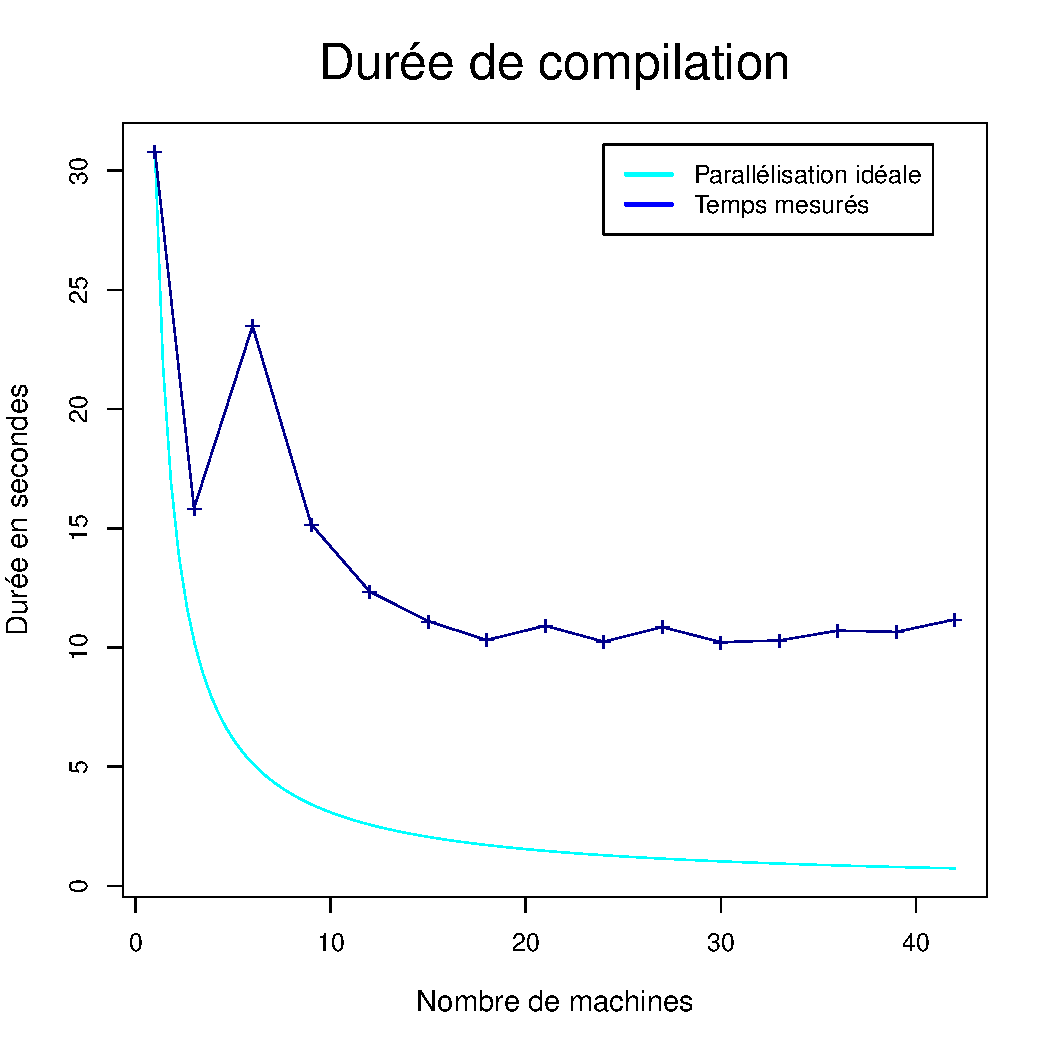
\includegraphics[scale=0.5]{res/sujet_makefiles_blender_259_Makefile_nth8.pdf}
% \end{wrapfigure}

% Alea jacta est.
% Alea jacta est.
% Alea jacta est.
% Alea jacta est.
% Alea jacta est.
% Alea jacta est.
% Alea jacta est.
% Alea jacta est.
% Alea jacta est.

\begin{center}
% \begin{figure}[ht!]
    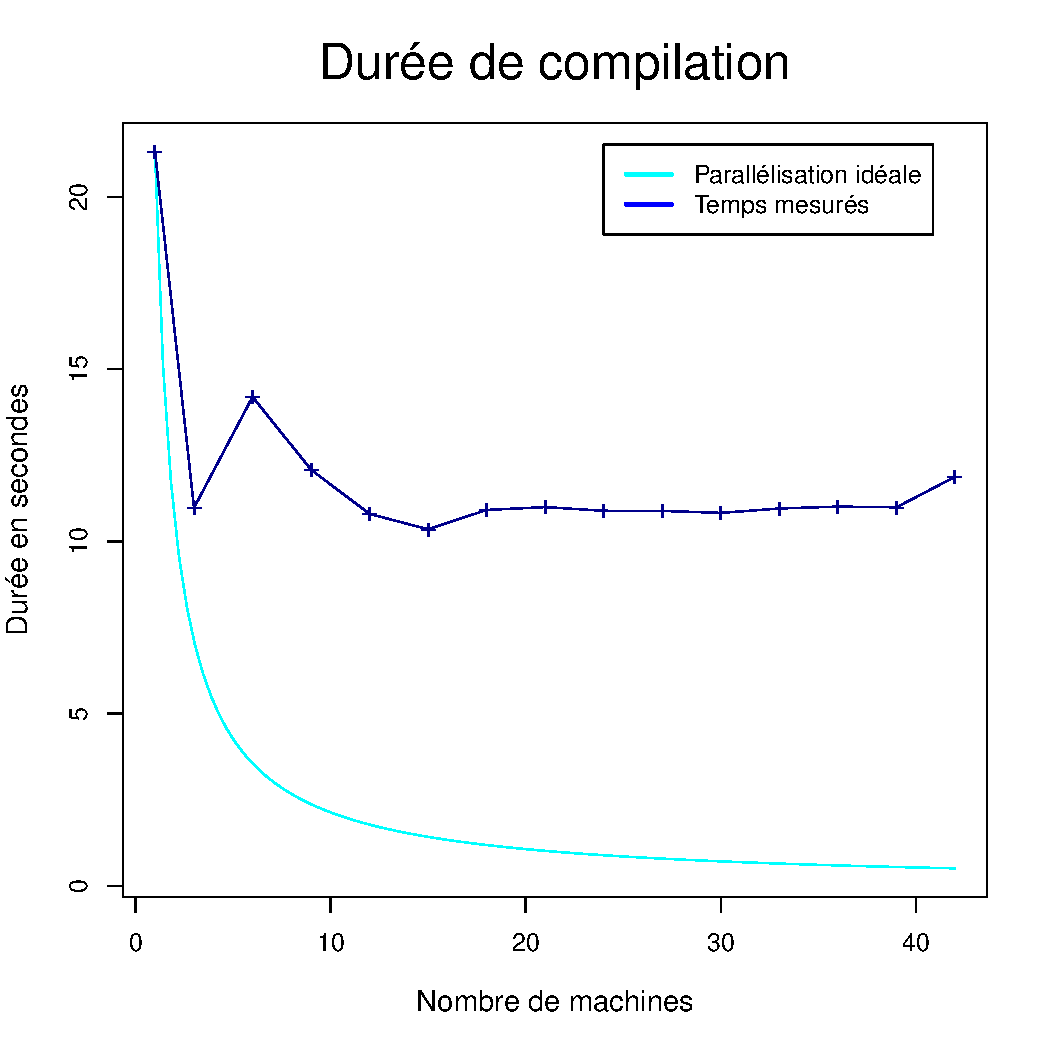
\includegraphics[scale=0.55]{res/sujet_makefiles_blender_249_Makefile_nth8.pdf}
% \caption{Diagramme des cas d'utilisation}
% \end{figure}
\end{center}


\subsubsection {Makefile-recurse}

\begin{center}
% \begin{figure}[ht!]
    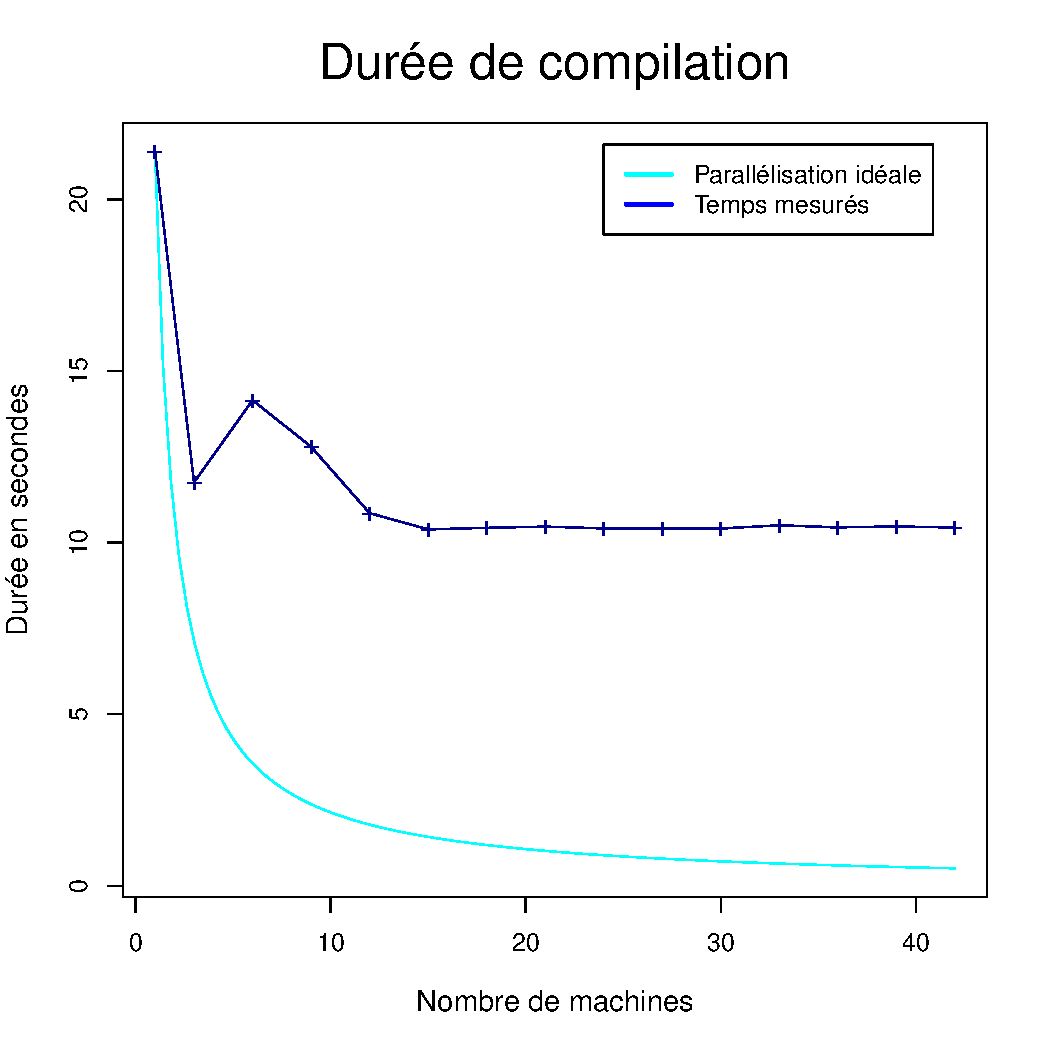
\includegraphics[scale=0.55]{res/sujet_makefiles_blender_249_Makefile-recurse_nth8.pdf}
% \caption{Diagramme des cas d'utilisation}
% \end{figure}
\end{center}


\subsection {Blender 2.59}


\begin{center}
% \begin{figure}[ht!]
    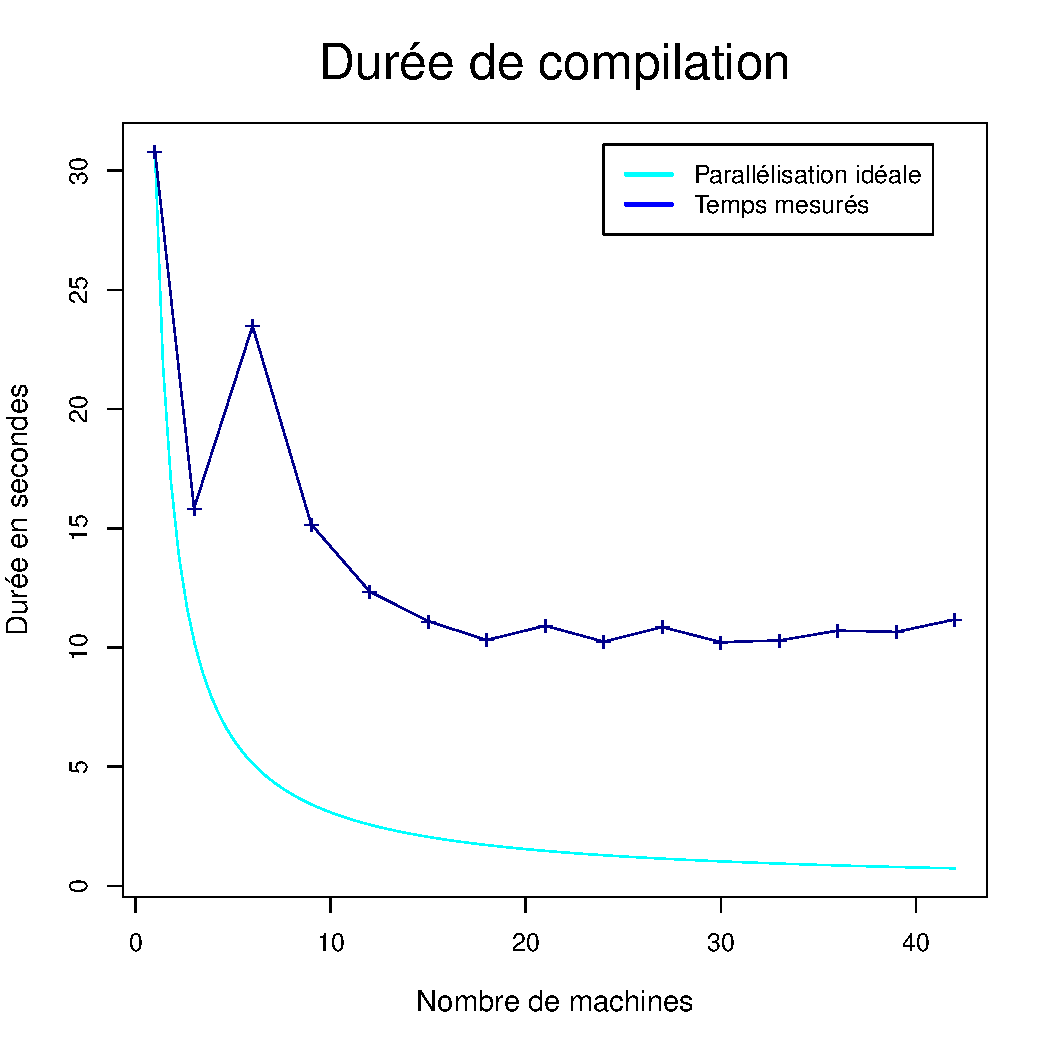
\includegraphics[scale=0.6]{res/sujet_makefiles_blender_259_Makefile_nth8.pdf}
% \caption{Diagramme des cas d'utilisation}
% \end{figure}
\end{center}



\subsection {Matrix}

\begin{center}
% \begin{figure}[ht!]
    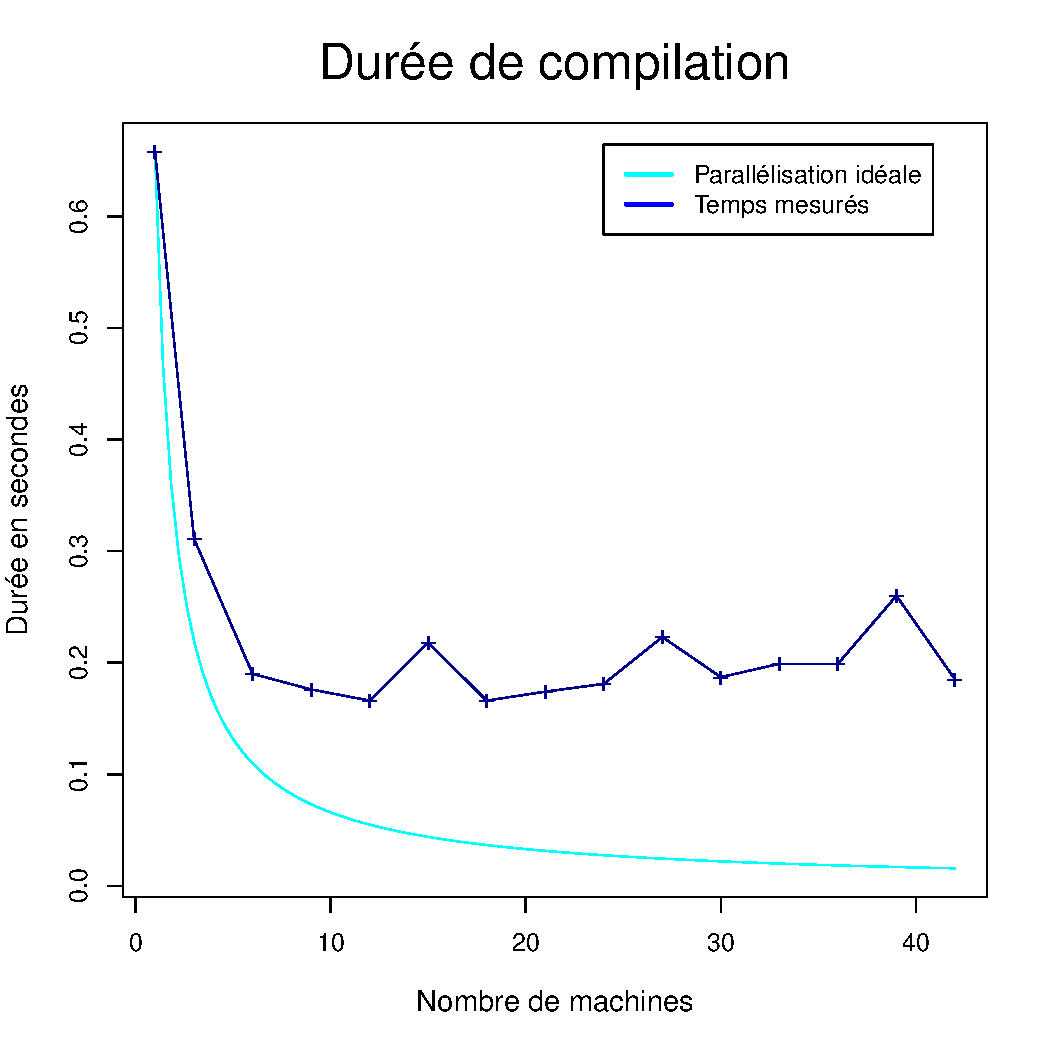
\includegraphics[scale=0.6]{res/sujet_makefiles_matrix_Makefile_nth8.pdf}
% \caption{Diagramme des cas d'utilisation}
% \end{figure}
\end{center}


\subsection {Premier}

\subsubsection {Makefile}

\begin{center}
% \begin{figure}[ht!]
    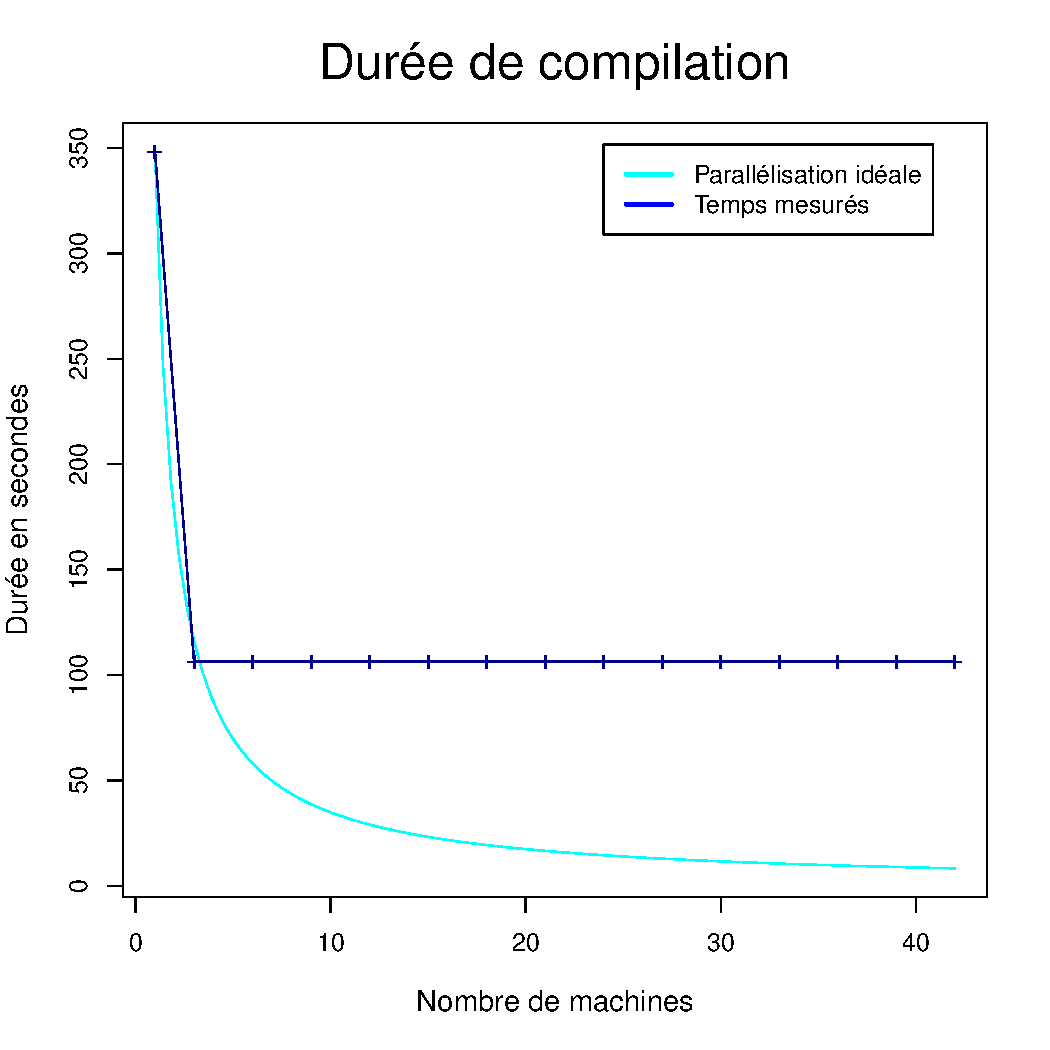
\includegraphics[scale=0.55]{res/sujet_makefiles_premier_Makefile_nth8.pdf}
% \caption{Diagramme des cas d'utilisation}
% \end{figure}
\end{center}


\subsubsection {Makefile-small}

\begin{center}
% \begin{figure}[ht!]
    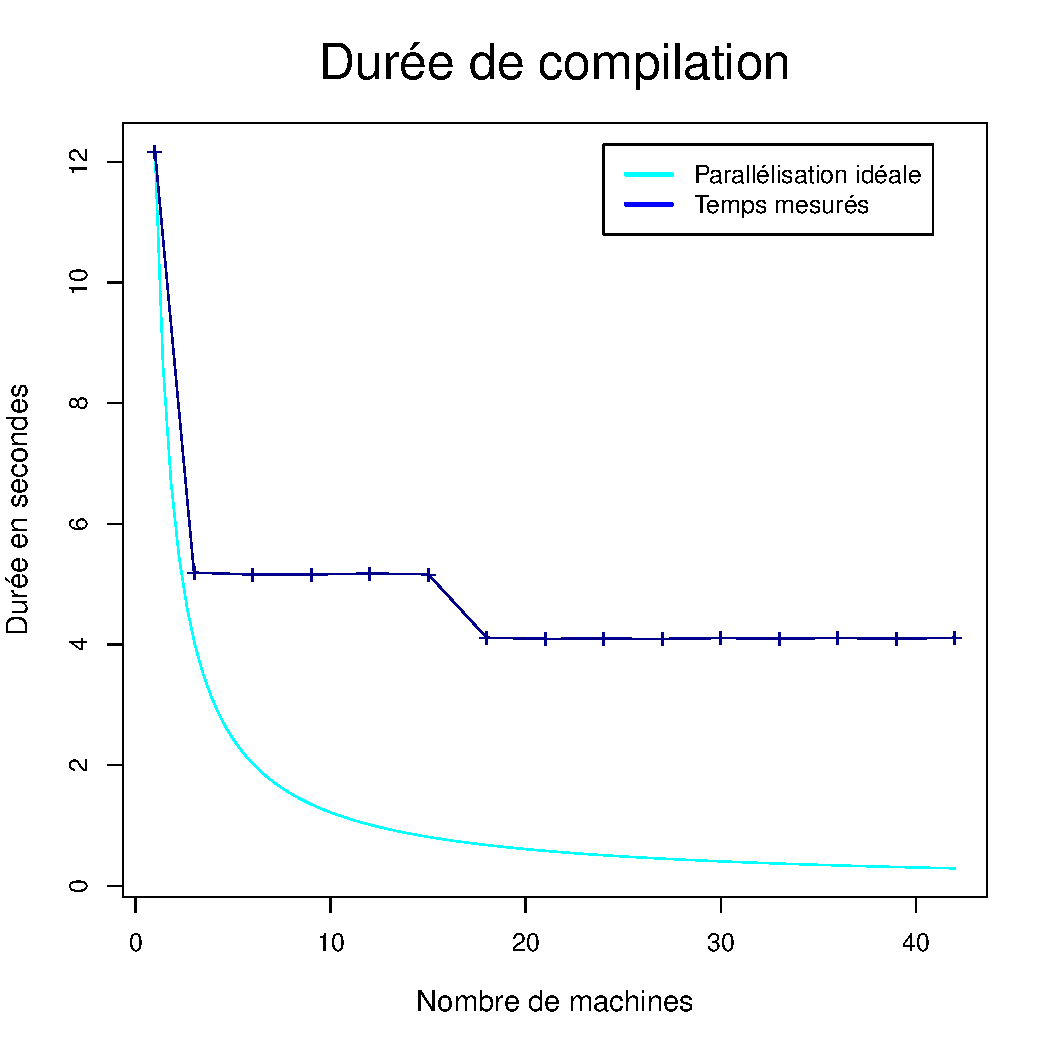
\includegraphics[scale=0.55]{res/sujet_makefiles_premier_Makefile-small_nth8.pdf}
% \caption{Diagramme des cas d'utilisation}
% \end{figure}
\end{center}


\end{document}


